% =====================================================================
%  Computational String Art — 중간발표 (Beamer)
%  수학과 예술: 스트링 아트의 계산적 생성
% =====================================================================
\documentclass[10pt,aspectratio=169]{beamer}

% ---- Theme -----------------------------------------------------------
\usetheme{Madrid}
\usecolortheme{seahorse}
\setbeamertemplate{navigation symbols}{}
\setbeamertemplate{footline}[frame number]

% ---- Korean / fonts --------------------------------------------------
\usepackage{kotex}

% ---- Math ------------------------------------------------------------
\usepackage{amsmath,amssymb,mathtools}

% ---- Graphics / layout -----------------------------------------------
\usepackage{graphicx}
\usepackage{booktabs}
\usepackage{tikz}
\usetikzlibrary{arrows.meta,positioning,calc,shapes.geometric}

% ---- Code listing ----------------------------------------------------
\usepackage{listings}
\usepackage{xcolor}
\lstset{
  language=Python,
  basicstyle=\ttfamily\tiny,
  keywordstyle=\color{blue!70!black}\bfseries,
  commentstyle=\color{gray!80!black},
  stringstyle=\color{red!60!black},
  showstringspaces=false,
  breaklines=true,
  frame=single,
  tabsize=4,
  numbers=left,
  numberstyle=\tiny\color{gray},
  numbersep=5pt
}

% ---- Meta info -------------------------------------------------------
\title[Computational String Art]{%
  \textbf{Computational String Art}\\[4pt]
  에너지 최소화 기반 스트링 아트 알고리즘}
\subtitle{수학과 예술 — 중간발표}
\author{김페이퍼}
\institute{한국과학영재학교}
\date{2026년 3월}

% =====================================================================
\begin{document}

% ── 표지 ──────────────────────────────────────────────
\begin{frame}
  \titlepage
\end{frame}

% ── 목차 ──────────────────────────────────────────────
\begin{frame}{목차}
  \tableofcontents
\end{frame}

% =================================================================
\section{프로젝트 개요}
% =================================================================

\begin{frame}{프로젝트 개요}
  \begin{block}{주제: 수학과 예술 — Computational String Art}
    입력 이미지를 \textbf{실(thread)과 핀(pin)}만으로 재현하는
    스트링 아트를 \textbf{컴퓨터 알고리즘}으로 자동 생성한다.
  \end{block}

  \vspace{0.3cm}
  \begin{columns}[T]
    \begin{column}{0.55\textwidth}
      \textbf{핵심 질문}
      \begin{itemize}
        \item 원형 프레임 위의 $N$개 핀 사이에 실을 어떤 순서로 연결하면
              원본 이미지에 가장 가까운 결과를 얻을 수 있는가?
        \item 수학적 최적화 기법을 어떻게 활용할 수 있는가?
      \end{itemize}
    \end{column}
    \begin{column}{0.4\textwidth}
      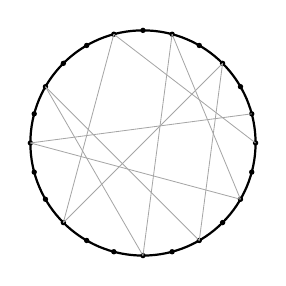
\begin{tikzpicture}[scale=0.65]
        \draw[thick] (0,0) circle (2.2);
        \foreach \i in {0,1,...,23} {
          \fill ({2.2*cos(\i*15)},{2.2*sin(\i*15)}) circle (1.5pt);
        }
        \foreach \a/\b in {0/7,7/15,15/3,3/20,20/10,10/18,18/5,5/22,22/12,12/1} {
          \draw[gray!70,line width=0.3pt]
            ({2.2*cos(\a*15)},{2.2*sin(\a*15)}) --
            ({2.2*cos(\b*15)},{2.2*sin(\b*15)});
        }
      \end{tikzpicture}
    \end{column}
  \end{columns}
\end{frame}

\begin{frame}{참고자료 및 배경}
  \begin{itemize}
    \item \textbf{주요 논문}: Birsak et al., \textit{``String Art: Towards
          Computational Fabrication of String Images''}, Eurographics 2018
    \item \textbf{추가 참고}: Bridges 2022 학회 논문 (수학과 예술의 연결)
    \item \textbf{기존 구현 분석}: \texttt{1st review.py} — 에너지 최소화
          기반 고급 알고리즘 (1,362줄)
    \item \textbf{보조 실험}: \texttt{fibonacci\_string\_art.py} — 피보나치
          수열 기반 핀 연결 패턴
    \item \textbf{기존 보고서}: \texttt{Untitled-1.tex} — 알고리즘 수학적
          분석 보고서
  \end{itemize}

  \vspace{0.3cm}
  \begin{alertblock}{핵심 아이디어}
    단순 ``가장 어두운 선 고르기''가 아니라,
    \textbf{물리 기반 투과율 모델 + 가중 $L^2$ 에너지 최적화 +
    다단계 개선 전략}을 결합한 정교한 접근
  \end{alertblock}
\end{frame}

% =================================================================
\section{알고리즘 전체 구조}
% =================================================================

\begin{frame}{알고리즘 5단계 개요}
  \begin{center}
  \begin{tikzpicture}[
    node distance=0.55cm,
    box/.style={rectangle,draw,rounded corners,align=center,
                minimum width=13cm,minimum height=0.65cm,font=\small,
                fill=blue!8},
    arr/.style={-{Stealth[length=2mm]},thick,blue!60!black}
  ]
    \node[box] (a) {1. \textbf{전처리}: 이미지 로드 → 그레이스케일 → 원형 마스크 → 에지 중요도 맵};
    \node[box,below=of a] (b) {2. \textbf{사전계산}: 핀 좌표 생성, 유효 선분 픽셀 캐시 (병렬)};
    \node[box,below=of b] (c) {3. \textbf{탐욕 구성}: $\Delta E$ 최대화 기반 순차 선택 + 2-step Lookahead};
    \node[box,below=of c] (d) {4. \textbf{정련(Refinement)}: 시퀀스 재생성, 각 선택 재평가 및 교체};
    \node[box,below=of d] (e) {5. \textbf{후처리}: 시퀀스 압축 + 시뮬레이티드 어닐링 (MCMC)};
    \draw[arr] (a) -- (b);
    \draw[arr] (b) -- (c);
    \draw[arr] (c) -- (d);
    \draw[arr] (d) -- (e);
  \end{tikzpicture}
  \end{center}
\end{frame}

% =================================================================
\section{수학적 모델}
% =================================================================

\begin{frame}{투과율(Transmittance) 곱셈 모델}
  \begin{block}{기존 단순 모델 vs.\ 구현 모델}
    \begin{itemize}
      \item 기존 단순: $R \leftarrow R - w\ell$ (가산적 감소, 과도 암화 문제)
      \item \textbf{구현}: Beer--Lambert 법칙 기반 \textbf{곱셈 모델}
    \end{itemize}
  \end{block}

  \vspace{0.3cm}
  \textbf{핵심 수식}:
  \begin{align}
    T(r,c) &\in [0,1], \quad R(r,c) = 255 \cdot T(r,c) \\[4pt]
    \text{선 추가 시:}\quad T'_i &= T_i \cdot (1 - \alpha \cdot v_i)
  \end{align}

  여기서:
  \begin{itemize}
    \item $T$: 투과율 (1 = 흰색, 0 = 완전 불투명)
    \item $\alpha$: 실 불투명도 (기본 0.08)
    \item $v_i$: 안티앨리어싱 가중치 (Xiaolin-Wu 알고리즘)
  \end{itemize}

  \vspace{0.2cm}
  $\Rightarrow$ 실이 겹칠수록 효과가 \textbf{자연스럽게 감소} (물리적 포화 반영)
\end{frame}

\begin{frame}{에너지 함수와 선택 점수}
  \textbf{최적화 목표} — 가중 $L^2$ 에러 최소화:
  \[
    E(T) = \sum_{r,c} W(r,c) \cdot \bigl(R(r,c) - I_{\text{target}}(r,c)\bigr)^2
  \]

  \vspace{0.2cm}
  \textbf{한 가닥 추가 시 에너지 감소량} (closed-form):
  \begin{align}
    d_i &= R_i - I_i \quad \text{(잔차, 양수 = 너무 밝음)} \\
    s_i &= R_i \cdot \alpha \cdot v_i \quad \text{(감쇠량)} \\[6pt]
    \Delta E &= \sum_i W_i \cdot s_i \cdot (2d_i - s_i)
  \end{align}

  \begin{itemize}
    \item $\Delta E > 0$: 에러 감소 (좋은 선택)
    \item $\Delta E \le 0$: 비개선 (선택하지 않음)
  \end{itemize}

  \vspace{0.2cm}
  \begin{exampleblock}{중요도 맵 $W$}
    Sobel 에지 검출 → 윤곽/디테일에 높은 가중치:
    $W(r,c) = (1 + \lambda \cdot E_{\text{edge}}(r,c)) \cdot M_{\text{circle}}$
  \end{exampleblock}
\end{frame}

% =================================================================
\section{핵심 알고리즘 상세}
% =================================================================

\begin{frame}{핀 기하학과 선분 사전계산}
  \begin{columns}[T]
    \begin{column}{0.55\textwidth}
      \textbf{핀 배치}:
      \[
        P_k = \left(\frac{M}{2} + r\cos\frac{2\pi k}{N},\;
              \frac{M}{2} + r\sin\frac{2\pi k}{N}\right)
      \]
      ($k = 0, \ldots, N{-}1$, $r = M/2 - 1$)

      \vspace{0.3cm}
      \textbf{유효 핀 쌍 조건}:
      \[
        d_{\text{arc}}(i,j) = \min(|i{-}j|, N{-}|i{-}j|) \ge \delta
      \]
      ($\delta = 20$: 너무 짧은 선 제거)

      \vspace{0.3cm}
      \textbf{Xiaolin-Wu 안티앨리어싱}:
      \begin{itemize}
        \item 각 선분의 픽셀 좌표 $(rr, cc)$ 및 강도 $val$ 사전계산
        \item \texttt{multiprocessing.Pool}로 병렬 처리
        \item 288핀 기준 약 37,000개 유효 선분
      \end{itemize}
    \end{column}
    \begin{column}{0.4\textwidth}
      \begin{tikzpicture}[scale=0.7]
        \draw[thick] (0,0) circle (2.5);
        \foreach \i in {0,1,...,11} {
          \fill[red!70!black] ({2.5*cos(\i*30)},{2.5*sin(\i*30)}) circle (2pt);
          \node[font=\tiny] at ({2.9*cos(\i*30)},{2.9*sin(\i*30)}) {\i};
        }
        \draw[blue!50,line width=0.5pt]
          ({2.5*cos(0)},{2.5*sin(0)}) -- ({2.5*cos(150)},{2.5*sin(150)});
        \draw[blue!50,line width=0.5pt]
          ({2.5*cos(30)},{2.5*sin(30)}) -- ({2.5*cos(210)},{2.5*sin(210)});
        \draw[red!30,line width=0.5pt,dashed]
          ({2.5*cos(0)},{2.5*sin(0)}) -- ({2.5*cos(30)},{2.5*sin(30)});
        \node[font=\tiny,red!70!black] at (0,-3.2) {빨간 점선: $d_{\text{arc}} < \delta$ (제외)};
      \end{tikzpicture}
    \end{column}
  \end{columns}
\end{frame}

\begin{frame}{탐욕 구성 (Phase 1)}
  \begin{enumerate}
    \item \textbf{시작 핀 자동 선택}:
      \[
        p_0 = \arg\max_p \max_{q \in \mathcal{N}(p)} \Delta E(p, q)
      \]
    \item \textbf{반복}: 현재 핀 $p_t$에서 모든 후보 $q$에 대해 $\Delta E$ 계산
    \item \textbf{재사용 페널티}: 같은 핀쌍 사용 횟수 $u$에 비례한 감쇄
    \item \textbf{2-step Beam Lookahead}:
      \begin{itemize}
        \item 상위 $K$개 후보에 대해 1-step 더 예측
        \item $\text{score} = \Delta E_{\text{reg}} + w \cdot \max(0, \Delta E_{\text{next}})$
      \end{itemize}
    \item \textbf{적용}: $T \leftarrow T \cdot (1 - \alpha v)$
  \end{enumerate}

  \vspace{0.3cm}
  \begin{block}{정지 조건}
    \begin{itemize}
      \item 최적 점수 $\le 0$ (즉시 정지)
      \item 추세 정체: 최근 평균이 초기 평균의 0.5\% 미만이 80회 초과 지속
    \end{itemize}
  \end{block}
\end{frame}

\begin{frame}{정련 및 후처리 (Phase 2--5)}
  \textbf{Phase 2: 정련 (Refinement)}
  \begin{itemize}
    \item 탐욕 시퀀스를 처음부터 \textbf{재생성}
    \item 각 단계에서 원래 목적지 $q_{\text{orig}}$ vs.\ 최선 대체 $q_{\text{best}}$ 비교
    \item $\Delta E(q_{\text{best}}) > \Delta E(q_{\text{orig}})$이면 교체
  \end{itemize}

  \vspace{0.3cm}
  \textbf{Phase 3: 시퀀스 압축 (Compression)}
  \begin{itemize}
    \item $(a \to b \to c)$ 패턴을 $(a \to c)$로 축약 (실 수 감소)
    \item 에너지 손실이 허용 범위 이내일 때만 적용
  \end{itemize}

  \vspace{0.3cm}
  \textbf{Phase 4: 시뮬레이티드 어닐링 (MCMC)}
  \begin{itemize}
    \item 전역 최적화: 노드 교체(replace), 삭제(delete), 삽입(insert)
    \item 온도 스케줄: $T_{\text{init}} = 5.0 \to T_{\text{end}} = 0.05$
    \item 50,000 스텝 동안 시퀀스 토폴로지 탐색
  \end{itemize}
\end{frame}

% =================================================================
\section{코드 구조}
% =================================================================

\begin{frame}[fragile]{코드 구조 — \texttt{1st review.py}}
  \begin{columns}[T]
    \begin{column}{0.48\textwidth}
      \textbf{주요 클래스}: \texttt{StringArt}
      \vspace{0.2cm}

      \begin{tabular}{ll}
        \toprule
        메서드 & 역할 \\
        \midrule
        \texttt{\_load\_image} & 이미지 전처리 \\
        \texttt{\_compute\_importance} & 중요도 맵 생성 \\
        \texttt{\_precompute\_lines} & 선분 픽셀 캐시 \\
        \texttt{\_line\_error\_reduction} & $\Delta E$ 계산 \\
        \texttt{\_best\_move\_with\_} & Beam 탐색 \\
        \quad\texttt{lookahead} & \\
        \texttt{\_compress\_sequence} & 시퀀스 압축 \\
        \texttt{\_simulated\_annealing} & MCMC 최적화 \\
        \texttt{run} & 전체 실행 \\
        \bottomrule
      \end{tabular}
    \end{column}
    \begin{column}{0.48\textwidth}
      \textbf{에너지 감소량 핵심 코드}:
      \begin{lstlisting}
R = 255.0 * transmittance[rr, cc]
T = self.target[rr, cc]
W = self.importance[rr, cc]
a = self.string_opacity * val

s = R * a           # darkening
d = R - T           # residual

score = np.sum(W * s * (2.0*d - s))
      \end{lstlisting}

      \vspace{0.2cm}
      \textbf{투과율 갱신}:
      \begin{lstlisting}
transmittance[rr, cc] *= (
    1.0 - self.string_opacity * val
)
      \end{lstlisting}
    \end{column}
  \end{columns}
\end{frame}

\begin{frame}{주요 파라미터}
  \begin{center}
  \small
  \begin{tabular}{lcp{7.5cm}}
    \toprule
    파라미터 & 기본값 & 의미 \\
    \midrule
    \texttt{num\_pins}    & 288   & 핀 개수 (해상도 $\uparrow$ = 표현력 $\uparrow$, 계산량 $\uparrow$) \\
    \texttt{max\_strings} & 10000 & 최대 실 수 (디테일 vs.\ 시간) \\
    \texttt{string\_opacity} & 0.08 & 실 불투명도 (너무 크면 과암화) \\
    \texttt{min\_pin\_distance} & 20 & 최소 핀 거리 (짧은 선 제거) \\
    \texttt{img\_size}    & 700   & 작업 해상도 ($700 \times 700$) \\
    \texttt{importance\_edge\_weight} & 1.5 & 에지 가중치 $\lambda$ \\
    \texttt{refinement\_rounds} & 1 & 정련 횟수 \\
    \texttt{lookahead\_width} & 24 & Beam 탐색 폭 $K$ \\
    \texttt{mcmc\_steps}  & 50000 & SA 탐색 스텝 수 \\
    \bottomrule
  \end{tabular}
  \end{center}
\end{frame}

% =================================================================
\section{보조 실험: 피보나치 스트링 아트}
% =================================================================

\begin{frame}[fragile]{피보나치 스트링 아트}
  \texttt{fibonacci\_string\_art.py}: 수학적 패턴 기반의 단순 스트링 아트

  \vspace{0.3cm}
  \begin{columns}[T]
    \begin{column}{0.5\textwidth}
      \textbf{원리}:
      \begin{itemize}
        \item 피보나치 수열로 핀 번호 생성:
          \[
            F(n) = (F(n{-}1) + F(n{-}2)) \bmod N
          \]
        \item 300개 핀, 2000개 실
        \item 이미지 재현이 아닌 \textbf{수학적 패턴 생성}
      \end{itemize}

      \vspace{0.2cm}
      \textbf{비교 포인트}:
      \begin{itemize}
        \item 에너지 최적화 없이 순수 수학 규칙
        \item 결과: 대칭적인 기하 패턴
        \item $\Rightarrow$ 최적화의 필요성을 보여줌
      \end{itemize}
    \end{column}
    \begin{column}{0.45\textwidth}
      \begin{lstlisting}
def generate_fibonacci_sequence(
    num_pins, max_steps):
    seq = [0, 1]
    for _ in range(max_steps - 2):
        next_pin = (seq[-1] + seq[-2])
                   % num_pins
        seq.append(next_pin)
    return seq
      \end{lstlisting}
    \end{column}
  \end{columns}
\end{frame}

% =================================================================
\section{병렬화 및 성능}
% =================================================================

\begin{frame}{병렬화 설계}
  코드는 두 종류의 병렬 처리를 활용:

  \vspace{0.3cm}
  \begin{columns}[T]
    \begin{column}{0.48\textwidth}
      \begin{block}{1. 프로세스 병렬 (\texttt{multiprocessing})}
        \begin{itemize}
          \item 대상: 선분 사전계산
          \item CPU-바운드 독립 태스크
          \item GIL 회피
          \item $\sim$37,000개 선분 동시 계산
        \end{itemize}
      \end{block}
    \end{column}
    \begin{column}{0.48\textwidth}
      \begin{block}{2. 스레드 병렬 (\texttt{ThreadPoolExecutor})}
        \begin{itemize}
          \item 대상: 후보 점수 평가
          \item 캐시 배열 조회 중심
          \item I/O 스타일 분할
          \item 매 반복 후보 동시 평가
        \end{itemize}
      \end{block}
    \end{column}
  \end{columns}

  \vspace{0.5cm}
  \textbf{대략적 복잡도}:
  \begin{align*}
    \text{사전계산} &\approx O(|\mathcal{E}| \cdot \bar{L}) \\
    \text{탐욕 구성} &\approx O(T \cdot K \cdot \bar{L}) \\
    \text{정련} &\approx O(R \cdot T \cdot K \cdot \bar{L})
  \end{align*}
  ($|\mathcal{E}|$: 유효 선분 수, $\bar{L}$: 평균 선분 길이, $T$: 실 수, $K$: 후보 수, $R$: 정련 라운드)
\end{frame}

% =================================================================
\section{수학적 원리 심화}
% =================================================================

\begin{frame}{에너지 감소량 유도}
  \textbf{증명}: 한 픽셀 $i$에서 선 추가 전후의 에러 변화

  \vspace{0.3cm}
  \begin{align}
    \text{추가 전 에러}: \quad & (d_i)^2 = (R_i - I_i)^2 \\[4pt]
    \text{추가 후}: \quad & R'_i = R_i(1 - \alpha v_i) \\
    & d'_i = R'_i - I_i = d_i - s_i \quad (s_i = R_i \alpha v_i) \\[4pt]
    \text{에러 감소}: \quad & (d_i)^2 - (d'_i)^2 = (d_i)^2 - (d_i - s_i)^2 \\
    & = 2 d_i s_i - s_i^2 = s_i(2d_i - s_i)
  \end{align}

  \vspace{0.3cm}
  \textbf{전체 감소량} (중요도 가중):
  \[
    \boxed{\Delta E = \sum_i W_i \cdot s_i \cdot (2d_i - s_i)}
  \]

  \vspace{0.2cm}
  $\Rightarrow$ 이 공식이 코드의 \texttt{\_line\_error\_reduction()} 함수와 \textbf{정확히 일치}
\end{frame}

\begin{frame}{희소 정규화 (Sparse Regularization)}
  단순 에너지 감소만으로는 실 수가 과도하게 증가 → \textbf{정규화 필요}

  \vspace{0.3cm}
  \textbf{정규화된 이득}:
  \[
    \Delta E_{\text{reg}} = \Delta E_{\text{raw}}
      - C_{\text{string}}
      - C_{\text{reuse}} \cdot u_{\text{pair}}
      - C_{\text{new}} \cdot \mathbb{1}[\text{새 핀}]
  \]

  \vspace{0.3cm}
  \begin{center}
  \small
  \begin{tabular}{lcp{6.5cm}}
    \toprule
    페널티 & 기본값 & 의미 \\
    \midrule
    $C_{\text{string}}$ & 3,000 & 실 추가 기본 비용 (해 크기 제어) \\
    $C_{\text{reuse}}$ & 1,200 & 핀쌍 재사용 비용 (다양성 확보) \\
    $C_{\text{new}}$ & 2,500 & 새 핀 도입 비용 (핀 수 제한) \\
    \bottomrule
  \end{tabular}
  \end{center}

  \vspace{0.3cm}
  $\Rightarrow$ $L_0$/$L_1$ 정규화 아이디어: 이미지 충실도와 해의 복잡도 사이 균형
\end{frame}

% =================================================================
\section{알고리즘 흐름도}
% =================================================================

\begin{frame}{전체 알고리즘 흐름도}
  \begin{center}
  \begin{tikzpicture}[
    node distance=0.5cm,
    box/.style={rectangle,draw,rounded corners,align=center,
                minimum width=6.5cm,minimum height=0.5cm,font=\tiny,
                fill=blue!5},
    decision/.style={diamond,draw,aspect=3,align=center,font=\tiny,
                     inner sep=1pt,fill=orange!10},
    arr/.style={-{Stealth[length=1.5mm]},thick,blue!50!black},
    scale=0.9, transform shape
  ]
    \node[box] (a) {입력 이미지 로드 + 원형 마스크 + 에지 중요도 맵 $W$};
    \node[box,below=of a] (b) {핀 좌표 $P_k$ 생성 + 유효 선분 $(rr,cc,val)$ 캐시};
    \node[box,below=of b] (c) {$T \equiv 1$, 시작 핀 $p_0 = \arg\max_p \max_q \Delta E$};
    \node[box,below=of c] (d) {후보별 $\Delta E$ 계산 + Beam Lookahead 선택};
    \node[decision,below=0.6cm of d] (e) {정지?};
    \node[box,left=1.5cm of e] (f) {$T \leftarrow T(1{-}\alpha v)$\\시퀀스 갱신};
    \node[box,right=1.5cm of e] (g) {정련 → 압축 → SA};
    \node[box,below=0.6cm of g] (h) {최종: $R=255T$, MSE/PSNR\\결과 저장};

    \draw[arr] (a) -- (b);
    \draw[arr] (b) -- (c);
    \draw[arr] (c) -- (d);
    \draw[arr] (d) -- (e);
    \draw[arr] (e) -- node[above,font=\tiny]{아니오} (f);
    \draw[arr] (f.north) |- (d.west);
    \draw[arr] (e) -- node[above,font=\tiny]{예} (g);
    \draw[arr] (g) -- (h);
  \end{tikzpicture}
  \end{center}
\end{frame}

% =================================================================
\section{출력 및 제작}
% =================================================================

\begin{frame}{출력물과 물리적 제작}
  알고리즘 출력물:
  \vspace{0.2cm}
  \begin{enumerate}
    \item \textbf{렌더링 이미지}: 투과율 $T$로부터 $R = 255T$ 계산
    \item \textbf{핀 시퀀스}: 연결 순서 (텍스트 파일)
    \item \textbf{물리 좌표}: 핀 위치를 mm 단위로 변환 (지름 600mm 기준)
    \item \textbf{핀 템플릿}: 고해상도(2000px) 핀 위치 도면
  \end{enumerate}

  \vspace{0.3cm}
  \begin{block}{품질 지표}
    \begin{itemize}
      \item \textbf{MSE} (Mean Squared Error): 원본과의 평균 제곱 오차
      \item \textbf{PSNR} (Peak Signal-to-Noise Ratio):
        $\text{PSNR} = 10 \log_{10}\!\left(\frac{255^2}{\text{MSE}}\right) \text{ dB}$
    \end{itemize}
  \end{block}

  \vspace{0.2cm}
  $\Rightarrow$ 디지털 결과를 그대로 \textbf{실물 스트링 아트}로 제작 가능
\end{frame}

% =================================================================
\section{최종 목표 및 향후 계획}
% =================================================================

\begin{frame}{최종 목표}
  \begin{block}{1. 알고리즘 완성 및 최적화}
    \begin{itemize}
      \item 에너지 최소화 스트링 아트 알고리즘 구현 완료
      \item 파라미터 튜닝을 통한 최적 결과 도출
      \item 다양한 입력 이미지에 대한 실험 및 비교
    \end{itemize}
  \end{block}

  \begin{block}{2. 수학적 분석}
    \begin{itemize}
      \item 투과율 곱셈 모델의 수학적 정당성 (Beer--Lambert 법칙)
      \item 에너지 감소량의 폐형식(closed-form) 유도
      \item 희소 정규화와 수렴성 분석
    \end{itemize}
  \end{block}

  \begin{block}{3. 물리적 제작}
    \begin{itemize}
      \item 알고리즘이 출력한 핀 시퀀스 / 좌표를 기반으로
            실제 스트링 아트 작품 제작
      \item 수학과 예술의 융합을 실물로 구현
    \end{itemize}
  \end{block}
\end{frame}

\begin{frame}{향후 계획}
  \begin{enumerate}
    \item \textbf{실험 확장}: 다양한 이미지 (인물, 풍경, 추상화)에 대한 결과 비교
    \item \textbf{파라미터 연구}: 핀 수, 불투명도, 정규화 비용의 영향 체계적 분석
    \item \textbf{색상 확장}: 다색 실을 이용한 컬러 스트링 아트 가능성 탐구
    \item \textbf{실물 제작}: 직경 60cm 원형 프레임에 288개 핀, 검정 실로 제작
    \item \textbf{최종 보고서}: 수학적 증명 + 실험 결과 + 제작 과정 문서화
  \end{enumerate}

  \vspace{0.4cm}
  \begin{alertblock}{핵심 메시지}
    수학적 최적화 기법(에너지 최소화, 정규화, MCMC)을
    예술적 표현에 적용하여, \textbf{``수학이 예술을 만드는''} 과정을
    이론과 실물 모두에서 보여주는 것이 최종 목표
  \end{alertblock}
\end{frame}

% ── 감사 슬라이드 ────────────────────────────────────
\begin{frame}
  \centering
  \vspace{2cm}
  {\Huge 감사합니다}\\[1cm]
  {\large 질문 및 토론}\\[0.5cm]
  {\small\texttt{KSA24-092/PAPERKIM}}
\end{frame}

\end{document}
